This experiment is to assess importance of careful memory management in multithreading of Rust. 
We implement merge-sort algorithm in two different ways. One is sharing source vector with Arc. 
The other is passing slice of source vector to child thread. 

Our merge-sort algorithm with vector is implemented with recursion. In these alogorithm, the splitting phase is merely aquiring index of split position, 
not actually splitting the source vector. At merge phase, merge function receives two independent vector and merge these into single new vector.

For sharing data implementaion, channel with sending data is used for multithreading method, because we want to ensure children threads return values before parent thread proceed execution. 
For passing slice implementation, we use scope method to enable children threads to receive reference from their parent ensuring the same purpose of sending data. 

Experiment performed is the comparison among sharing data and passing slice implementations to see the impact of Arc, Atomic reference conuting, to runtime performance.
These two implementations are theoritically the same operations other than using or not using Arc to share data. 
This comparison can effectively show how important careful memory management is in multithreading computation in Rust. 
In another word, how atomic reference counting can cost for computation in Rust programming.

The figure shows the result of 
An atomic reference count of the shareable vector is passed to every recursion steps and 


\begin{figure}[htb]
    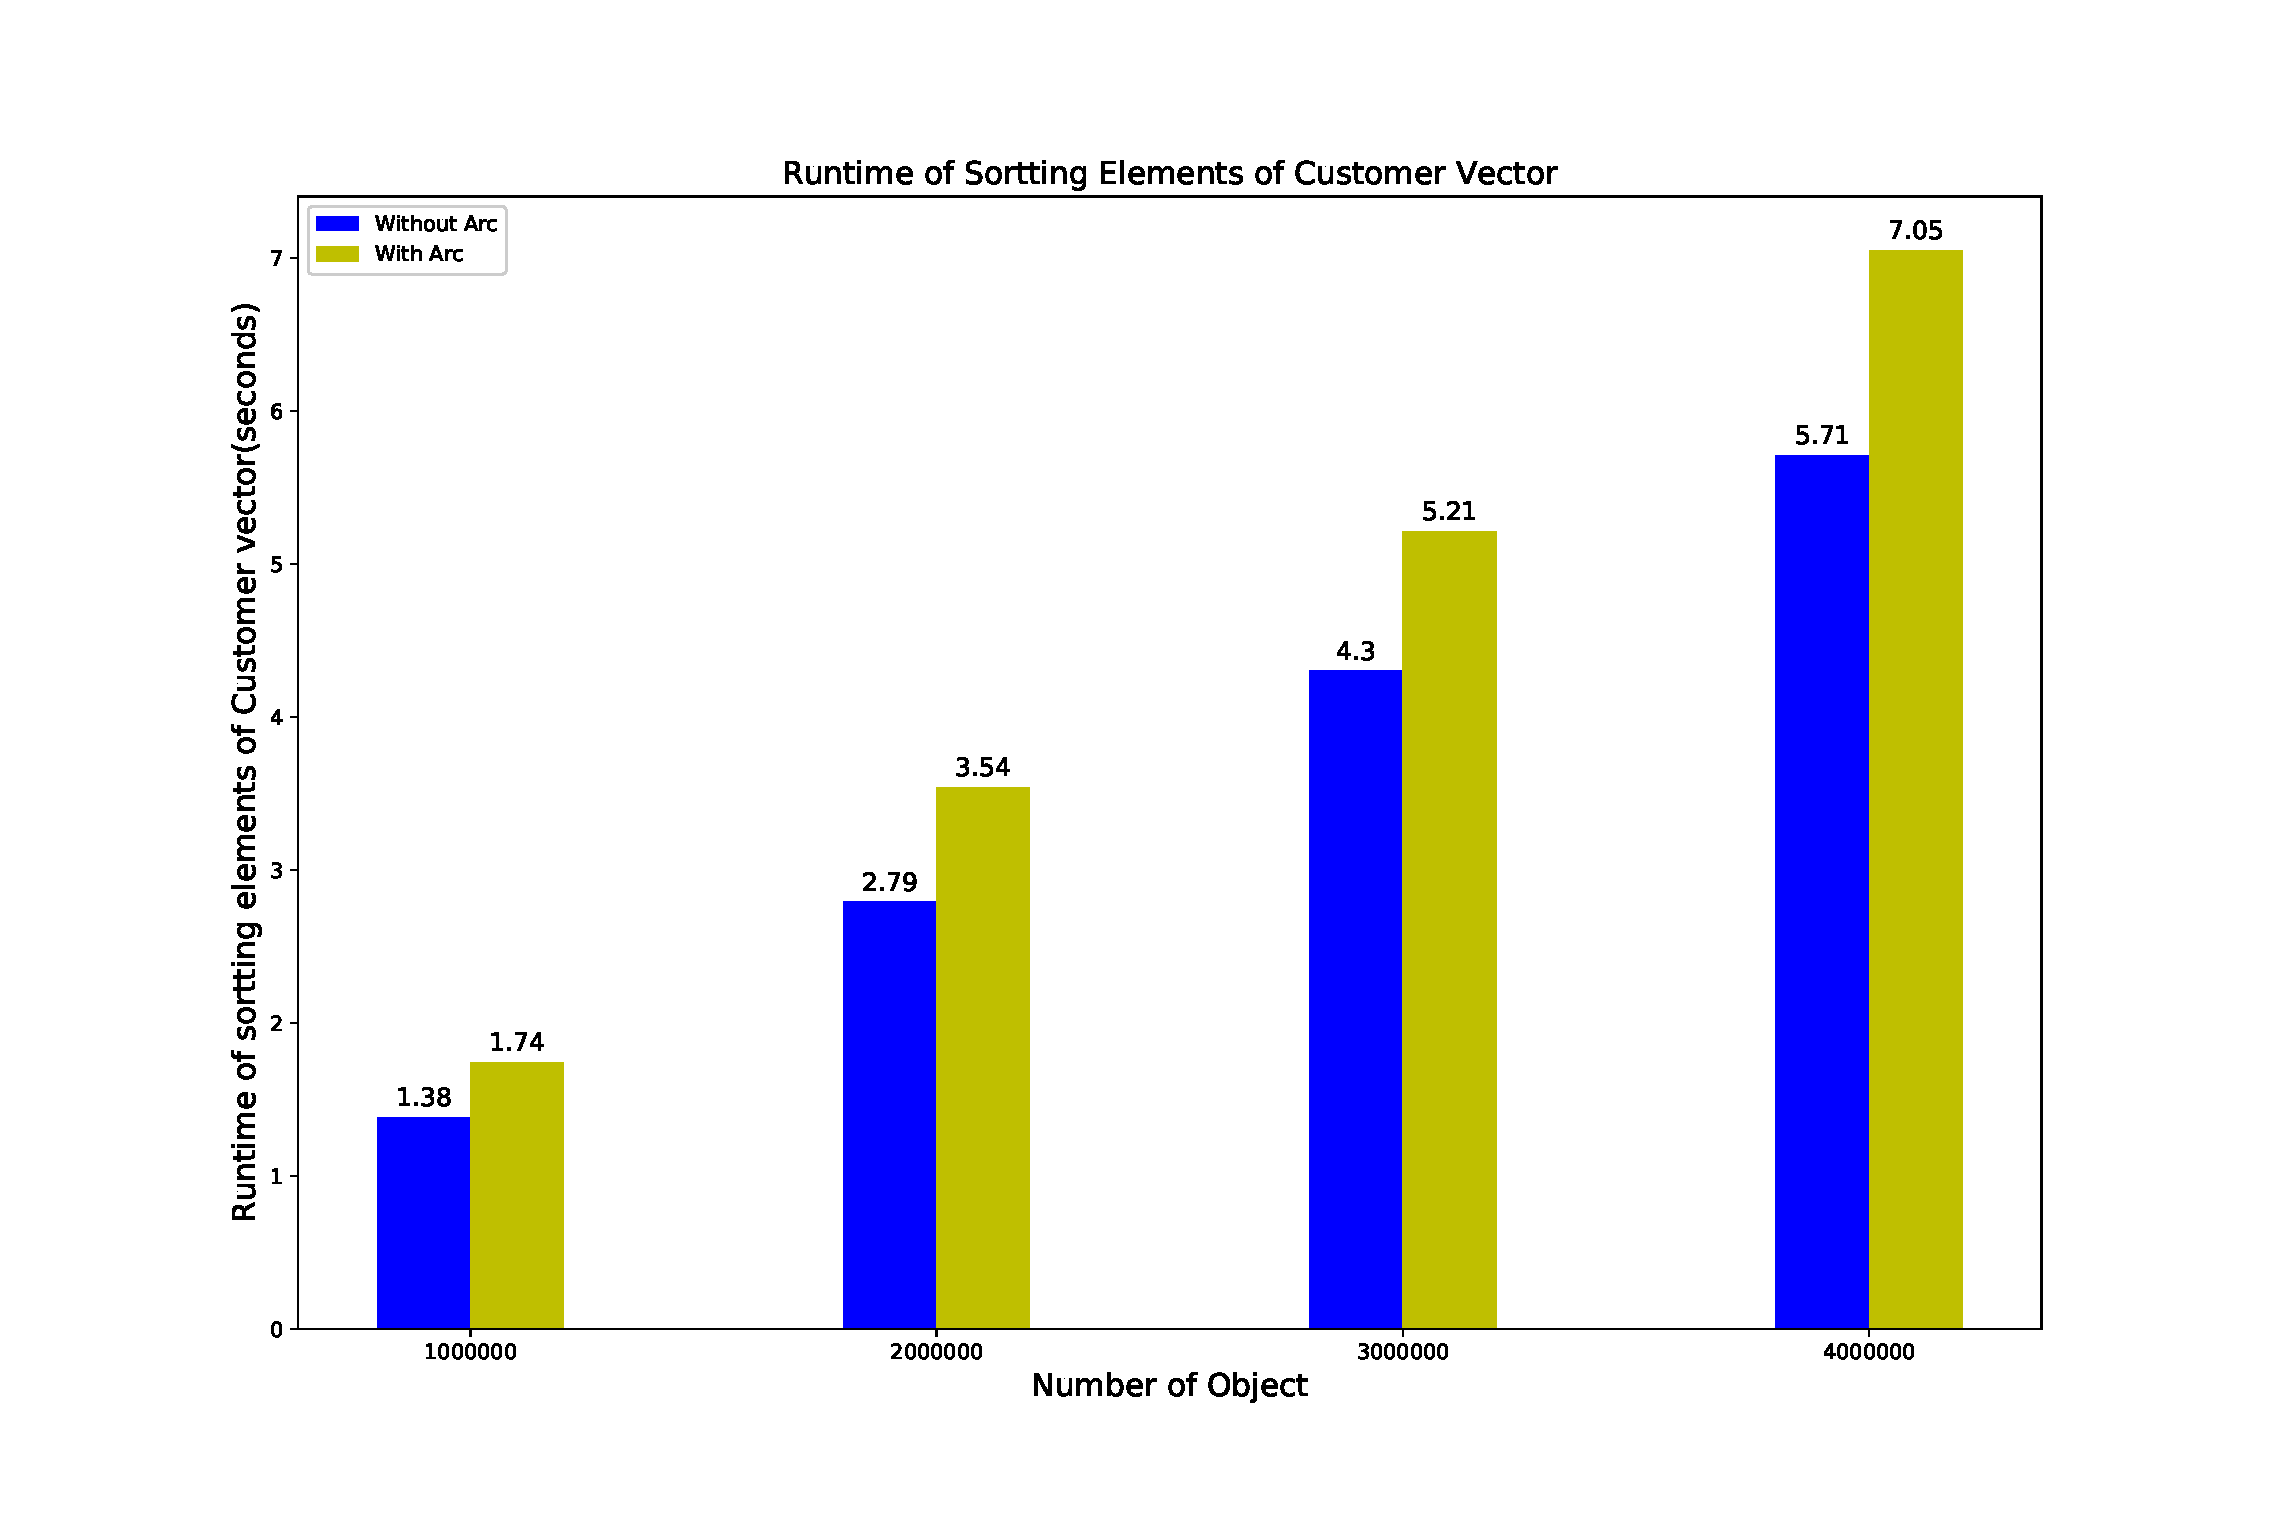
\includegraphics[width=15cm]{rust_merge_sort.eps}
    \caption{Runtime of Sortting Elements of Customer Vector}
    \label{fig:Sampling}
\end{figure}



The other is LinkedList implementation other than vector.
The linkedlist implementation is different from another two. This algorithm is inplace sorting so that it does not de/allocate memory during execution. 
The comparison among vector and linkedlist implementations can show trade-off between contiguous memory access and inplace non memory de/allocation. 
Experiment with Java linkedlist implementation can be interesting, because Java GC is severe problem when number of object is large. 